\documentclass[../main.tex]{subfiles}

\firstpageheader{6.042}{Recitation Problems 10}{Page \thepage\ of \numpages}
\runningheader{6.042}{Recitation Problems 10}{Page \thepage\ of \numpages}

\begin{document}

\begin{questions}

  \question Analysis of Two Networks
  \begin{solution}
    \begin{center}
      \begin{tabular}{c|c|c|c|c}
      network & \# switches & switch size  & diameter & max congestion \\
      \hline
      5-path  & $5$         & $3 \times 3$ & $6$      & $5$            \\
      \hline
      4-cycle & $4$         & $3 \times 3$ & $4$      & $3$            \\
      \end{tabular}
    \end{center}
  \end{solution}

  \question Routing in a Benes Network
  \begin{parts}

    \part Find the two subnetworks of size $N=4$ in the Benes networks of size $N=8$.
    \begin{solution}
      (\textit{skipped})
    \end{solution}

    \part Construct a constraint graph with dashed edges for packets that potentially collide in the second column of switches.
    \begin{solution}

      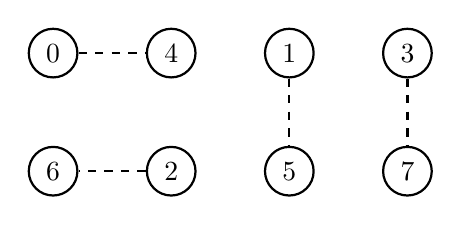
\begin{tikzpicture}[node distance={15mm}, thick, main/.style = {draw, circle}] 
      \node[main] (0) {$0$}; 
      \node[main] (4) [right of=0] {$4$}; 
      \node[main] (1) [right of=4] {$1$}; 
      \node[main] (5) [below of=1] {$5$}; 
      \node[main] (6) [below of=0] {$6$}; 
      \node[main] (2) [right of=6] {$2$}; 
      \node[main] (3) [right of=1] {$3$}; 
      \node[main] (7) [below of=3] {$7$}; 

      \draw[-] [dashed] (0) to (4);
      \draw[-] [dashed] (1) to (5);
      \draw[-] [dashed] (2) to (6);
      \draw[-] [dashed] (3) to (7);
      \end{tikzpicture}
    \end{solution}

    \part Add a solid edge in your graph between each pair of packets that can not go through the same subnetwork because a collision would occur in the next-to-last column of switches.
    \begin{solution}

      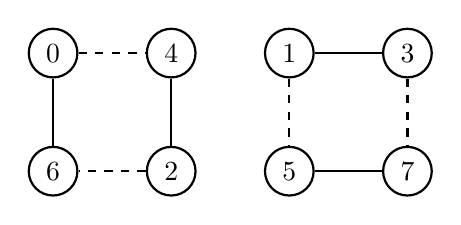
\begin{tikzpicture}[node distance={15mm}, thick, main/.style = {draw, circle}] 
      \node[main] (0) {$0$}; 
      \node[main] (4) [right of=0] {$4$}; 
      \node[main] (1) [right of=4] {$1$}; 
      \node[main] (5) [below of=1] {$5$}; 
      \node[main] (6) [below of=0] {$6$}; 
      \node[main] (2) [right of=6] {$2$}; 
      \node[main] (3) [right of=1] {$3$}; 
      \node[main] (7) [below of=3] {$7$}; 

      \draw[-] [dashed] (0) to (4);
      \draw[-] [dashed] (1) to (5);
      \draw[-] [dashed] (2) to (6);
      \draw[-] [dashed] (3) to (7);

      \draw[-] (5) to (7);
      \draw[-] (1) to (3);
      \draw[-] (2) to (4);
      \draw[-] (0) to (6);
      \end{tikzpicture}
    \end{solution}

    \part Color the vertices of your graph red and blue so that adjacent vertices get different colors. Why must this be possible, regardless of the permutation $\pi$?
    \begin{solution}

      \newcommand{\red}{rgb,255:red,255;green,145;blue,105}
      \newcommand{\blue}{rgb,255:red,133;green,190;blue,255}

      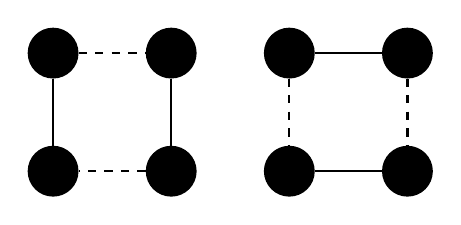
\begin{tikzpicture}[node distance={15mm}, thick, main/.style = {draw, circle}] 
      \node[main,fill={\red }] (0)              {$0$}; 
      \node[main,fill={\blue}] (4) [right of=0] {$4$}; 
      \node[main,fill={\red }] (1) [right of=4] {$1$}; 
      \node[main,fill={\blue}] (5) [below of=1] {$5$}; 
      \node[main,fill={\blue}] (6) [below of=0] {$6$}; 
      \node[main,fill={\red }] (2) [right of=6] {$2$}; 
      \node[main,fill={\blue}] (3) [right of=1] {$3$}; 
      \node[main,fill={\red }] (7) [below of=3] {$7$}; 

      \draw[-] [dashed] (0) to (4);
      \draw[-] [dashed] (1) to (5);
      \draw[-] [dashed] (2) to (6);
      \draw[-] [dashed] (3) to (7);

      \draw[-] (5) to (7);
      \draw[-] (1) to (3);
      \draw[-] (2) to (4);
      \draw[-] (0) to (6);
      \end{tikzpicture}

      A 2-coloring is always possible because the graph has even number of nodes and each node must be part of a cycle (due to the structure of a Benes network). This means every cycle has even length, thus it is 2-colorable. $\blacksquare$
    \end{solution}

    \part Suppose that red vertices correspond to packets routed through the upper subnetwork and blue vertices correspond to packets routed through the lower subnetwork. On the attached copy of the Benes network, highlight the first and last edge traversed by each packet.
    \begin{solution}

      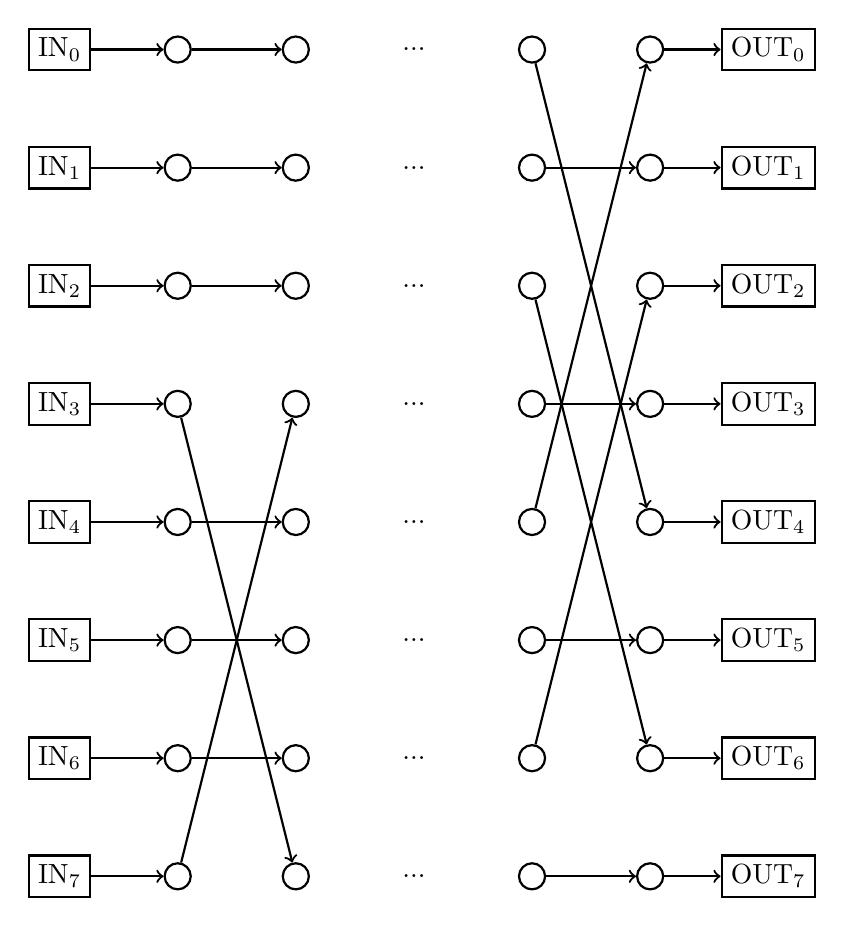
\begin{tikzpicture}[node distance={15mm}, thick, switch/.style = {draw, circle}, terminal/.style = {draw}] 

      \node[terminal] (IN_0) {IN$_0$}; 

      \foreach \i [evaluate=\i as \prev using {int(\i-1)}] in {1, ..., 7}
        \node[terminal] (IN_\i) [below of=IN_\prev] {IN$_\i$};

      \foreach \i in {0, ..., 7}
        \node[switch] (SW_0_\i) [right of=IN_\i] {};

      \foreach \i in {0, ..., 7}
        \node[switch] (SW_1_\i) [right of=SW_0_\i] {};

      \foreach \i in {0, ..., 7}
        \draw[->] (IN_\i) to (SW_0_\i);

      \draw[->] (SW_0_0) to (SW_1_0);
      \draw[->] (SW_0_1) to (SW_1_1);
      \draw[->] (SW_0_2) to (SW_1_2);
      \draw[->] (SW_0_3) to (SW_1_7);
      \draw[->] (SW_0_4) to (SW_1_4);
      \draw[->] (SW_0_5) to (SW_1_5);
      \draw[->] (SW_0_6) to (SW_1_6);
      \draw[->] (SW_0_7) to (SW_1_3);

      \foreach \i in {0, ..., 7}
        \node (PL_\i) [right of=SW_1_\i] {...};

      \foreach \i in {0, ..., 7}
        \node[switch] (SW_2_\i) [right of=PL_\i] {};

      \foreach \i in {0, ..., 7}
        \node[switch] (SW_3_\i) [right of=SW_2_\i] {};

      \foreach \i in {0, ..., 7}
        \node[terminal] (OUT_\i) [right of=SW_3_\i] {OUT$_\i$};

      \foreach \i in {0, ..., 7}
        \draw[->] (SW_3_\i) to (OUT_\i);

      \draw[->] (SW_2_4) to (SW_3_0);
      \draw[->] (SW_2_1) to (SW_3_1);
      \draw[->] (SW_2_6) to (SW_3_2);
      \draw[->] (SW_2_3) to (SW_3_3);
      \draw[->] (SW_2_0) to (SW_3_4);
      \draw[->] (SW_2_5) to (SW_3_5);
      \draw[->] (SW_2_2) to (SW_3_6);
      \draw[->] (SW_2_7) to (SW_3_7);

      \end{tikzpicture}
    \end{solution}

    \pagebreak
    \part All that remains is to route packets through the upper and lower subnetworks. One way to do this is by applying the procedure described above recursively on each subnetwork. However, since the remaining problems are small, see if you can complete all the paths on your own.
    \begin{solution}

      Upper subnetwork:

      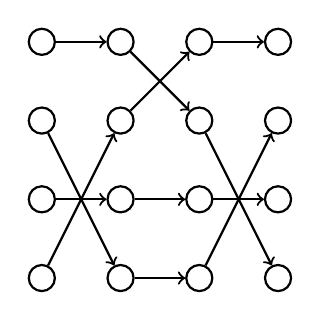
\begin{tikzpicture}[node distance={10mm}, thick, switch/.style = {draw, circle}] 

      \node[switch] (SW_0_0) {};

      \foreach \i [evaluate=\i as \prev using {int(\i-1)}] in {1, ..., 3}
        \node[switch] (SW_0_\i) [below of=SW_0_\prev] {};

      \foreach \col [evaluate=\col as \prevcol using {int(\col-1)}] in {1, ..., 3}
        \foreach \row in {0, ..., 3} 
          \node[switch] (SW_\col_\row) [right of=SW_\prevcol_\row] {};

      \draw[->] (SW_0_0) to (SW_1_0);
      \draw[->] (SW_1_0) to (SW_2_1);
      \draw[->] (SW_2_1) to (SW_3_3);

      \draw[->] (SW_0_1) to (SW_1_3);
      \draw[->] (SW_1_3) to (SW_2_3);
      \draw[->] (SW_2_3) to (SW_3_1);

      \draw[->] (SW_0_2) to (SW_1_2);
      \draw[->] (SW_1_2) to (SW_2_2);
      \draw[->] (SW_2_2) to (SW_3_2);

      \draw[->] (SW_0_3) to (SW_1_1);
      \draw[->] (SW_1_1) to (SW_2_0);
      \draw[->] (SW_2_0) to (SW_3_0);

      \end{tikzpicture}

      Lower subnetwork:

      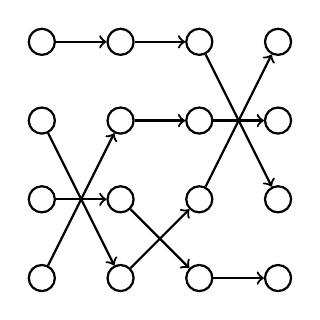
\begin{tikzpicture}[node distance={10mm}, thick, switch/.style = {draw, circle}] 

      \node[switch] (SW_0_0) {};

      \foreach \i [evaluate=\i as \prev using {int(\i-1)}] in {1, ..., 3}
        \node[switch] (SW_0_\i) [below of=SW_0_\prev] {};

      \foreach \col [evaluate=\col as \prevcol using {int(\col-1)}] in {1, ..., 3}
        \foreach \row in {0, ..., 3} 
          \node[switch] (SW_\col_\row) [right of=SW_\prevcol_\row] {};

      \draw[->] (SW_0_0) to (SW_1_0);
      \draw[->] (SW_1_0) to (SW_2_0);
      \draw[->] (SW_2_0) to (SW_3_2);

      \draw[->] (SW_0_1) to (SW_1_3);
      \draw[->] (SW_1_3) to (SW_2_2);
      \draw[->] (SW_2_2) to (SW_3_0);

      \draw[->] (SW_0_2) to (SW_1_2);
      \draw[->] (SW_1_2) to (SW_2_3);
      \draw[->] (SW_2_3) to (SW_3_3);

      \draw[->] (SW_0_3) to (SW_1_1);
      \draw[->] (SW_1_1) to (SW_2_1);
      \draw[->] (SW_2_1) to (SW_3_1);

      \end{tikzpicture}
    \end{solution}

  \end{parts}

\end{questions}
\end{document}
